% Part: model-theory
% Chapter: interpolation
% Section: separation

\documentclass[../../../include/open-logic-section]{subfiles}

\begin{document}

\olfileid[tr]{mod}{int}{sep}

\olsection{\printtoken{P}{sentence} Ayırma}

Aradeğerleme teoreminin ispatına geçmeden önce biraz hazırlık gerekir.
$!A$ ile $!B$ için bir aradeğerleyen, $!A\Entails !C$ ve
$!C\Entails !B$ olacak !!a{sentence}~$!C$ ifadesidir. Karşıt-ters
gereği ikincisi, $\lnot !B\Entails\lnot !C$ olmasına denktir. Bu
özelliğe sahip !!^a{sentence}~$!C$ ifadesinin $!A$ ile $\lnot !B$
ifadelerini \emph{ayırdığı} söylenir. Dolayısıyla $!A$ ile $!B$ için
bir aradeğerleyen bulmak, $!A$ ile $\lnot !B$'yi ayıran !!a{sentence}
bulmak demektir. Çoğu kez olduğu gibi bir genellemeyi, iki
!!{sentence}s \emph{kümesini} ayıran bir tümceyi ele almak yararlı
olacaktır.

\begin{defn}
Bir $!C$ tümcesi, ancak ve ancak $\Gamma\Entails !C$ ve
$\Delta\Entails\lnot !C$ ise $\Gamma$ ile $\Delta$ tümce kümelerini
\emph{ayırır}. Böyle bir !!{sentence} yoksa $\Gamma$ ile $\Delta$
\emph{ayrılamazdır}.
\end{defn}

$\Gamma$, $\Delta$ ve $!C$ model sınıfları arasındaki içerme ilişkileri
aşağıda gösterilmiştir:
\begin{figure}[h]
  \centering
  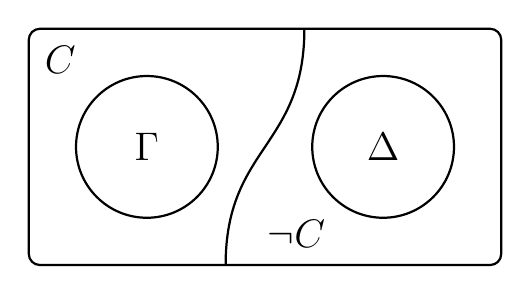
\begin{tikzpicture}[node distance=2cm, auto, thick]
    \draw [rounded corners] (0,0) -- (6,0) -- (6,3) -- (0,3) --  cycle;
    \draw (1.5,1.5) circle (0.9cm);
    \draw (4.5,1.5) circle (0.9cm);
    \path node at (1.5,1.5) {\Large $\Gamma$};
    \path node at (4.5,1.5) {\Large $\Delta$};
    \path node at (0.4,2.6) {\Large $\formula{C}$};
    \path node at (3.4,0.4) {\Large $\lnot \formula{C}$};
    \draw (2.5,0) .. controls (2.5,1.5) and (3.5,1.5) .. (3.5,3);
  \end{tikzpicture}
  \caption{$!C$, $\Gamma$ ile $\Delta$ kümelerini ayırır.}
  \ollabel{fig:sep}
\end{figure}

\begin{lem}\ollabel{lem:sep1}
$\Lang L_0$, hem $\Gamma$ hem $\Delta$ içinde geçen bütün
!!{constant}, !!{function} ve !!{predicate} simgelerini ($\doteq$
dışında) içeren dil olsun; $\Lang L'_0$ ise her $n\geq0$ için sonsuz
sayıda yeni !!{constant}s~$\Obj c_n$ eklenerek elde edilsin. $\Gamma$
ile $\Delta$, $\Lang L_0$ içinde ayrılamazsa $\Lang L'_0$ içinde de
ayrılamaz.
\end{lem}

\begin{proof}
Dolaylı ilerleyelim: Çelişki elde etmek üzere $\Gamma$ ile $\Delta$'nın
$\Lang L'_0$ içinde ayrıldığını varsayalım. O zaman bazı
$!C\in\Lang L_0$ için
$\Gamma\Entails\Subst{!C}{c}{x}$ ve
$\Delta\Entails\lnot\Subst{!C}{c}{x}$ olur (burada $c$ yeni bir
!!{constant}; $!C$ içinde birden çok yeni !!{constant} bulunan durum
benzerdir). Tıkızlık gereği $\Gamma$ ve $\Delta$ kümelerinin sonlu alt
kümeleri $\Gamma_0$ ile $\Delta_0$ vardır ve
$\Gamma_0\Entails\Subst{!C}{c}{x}$,
$\Delta_0\Entails\lnot\Subst{!C}{c}{x}$. $!G$, $\Gamma_0$ içindeki
bütün !!{formula}s ifadelerinin; $!H$ ise $\Delta_0$ içindekilerin
birleşimi olsun. O zaman
\begin{align*}
  !G & \Entails \Subst{!C}{c}{x}, &
  !H & \Entails \lnot \Subst{!C}{c}{x}.
\end{align*}
Birinciden genelleme yoluyla $!G\Entails\lforall[x][!C]$ elde edilir.
İkinciden karşıt-ters yoluyla
$\Subst{!C}{c}{x}\Entails\lnot !H$ ve dolayısıyla
$\lforall[x][!C]\Entails\lnot !H$ elde edilir. Yeniden karşıt-ters
$!H\Entails\lnot\lforall[x][!C]$ verir. Tekdüzelik gereği
\begin{align*}
  \Gamma &\Entails \lforall[x][!C], &
  \Delta &\Entails \lnot \lforall[x][!C].
\end{align*}
Dolayısıyla $\lforall[x][!C]$, $\Gamma$ ile $\Delta$'yı
$\Lang L_0$ içinde ayırır.
\end{proof}

\begin{lem}\ollabel{lem:sep2}
$\Gamma\cup\{\lexists[x][!S]\}$ ile $\Delta$ ayrılamaz ve $c$,
$\Gamma$, $\Delta$ ya da $!S$ içinde geçmeyen yeni bir !!{constant}
olsun. O zaman
$\Gamma\cup\{\lexists[x][!S],\Subst{!S}{c}{x}\}$ ile $\Delta$ da
ayrılamazdır.
\end{lem}

\begin{proof}
Çelişki için $!C$'nin
$\Gamma\cup\{\lexists[x][!S],\Subst{!S}{c}{x}\}$ ile $\Delta$'yı
ayırdığını, fakat $\Gamma\cup\{\lexists[x][!S]\}$ ile $\Delta$'nın
ayrılamaz olduğunu varsayalım. İki durumu ayırıyoruz:
\begin{enumerate}
\item $c$, $!C$ içinde geçmiyorsa
  $\Gamma\cup\{\lexists[x][!S],\lnot !C\}$ sağlanabilirdir (aksi halde
  $!C$, $\Gamma\cup\{\lexists[x][!S]\}$ ile $\Delta$'yı ayırırdı).
  $\Subst{!S}{c}{x}$ eklendiğinde de sağlanabilir kalır; dolayısıyla
  $!C$ aslında
  $\Gamma\cup\{\lexists[x][!S],\Subst{!S}{c}{x}\}$ ile $\Delta$'yı
  ayırmaz.
\item $c$, $!C$ içinde geçiyorsa $!C$, $\Subst{!C}{c}{x}$ biçimindedir.
  O zaman
  \[
  \Gamma \cup \{ \lexists[x][!S], \Subst{!S}{c}{x}\}
  \Entails \Subst{!C}{c}{x}.
  \]
  Tümdengelim teoremi ve genelleme yoluyla
  $\Gamma,\lexists[x][!S]\Entails\lforall[x][(!S\lif !C)]$ ve son
  olarak
  $\Gamma\cup\{\lexists[x][!S]\}\Entails\lexists[x][!C]$ elde edilir.
  Öte yandan $\Delta\Entails\lnot\Subst{!C}{c}{x}$ ve genelleme
  yoluyla $\Delta\Entails\lnot\lexists[x][!C]$. Böylece
  $\Gamma\cup\{\lexists[x][!S]\}$ ile $\Delta$ ayrılabilir olur; bu
  bir çelişkidir.
\end{enumerate}
\end{proof}

\end{document}
